This chapter presents the description of the simulations used for the current research. The objective of the simulation is to estimate the amplitude and frequency of the resultant generated wave post mixing. This is primarily due to the non-linear behaviour of the material in the mixing zone. The following are the steps followed to achieve this objective.

% Fancy Graphic Explaining What I will be doing%

\section{2D FDTD Simulation in Cartesian Coordinates}
Finite Difference Time Domain (FDTD) method is widely used to solve wave propagation problems. In the present work the FDTD algorithm is implemented in 2D Orthogonal Cartesian Coordinates. \cite{yee}
\section{Governing Equations}
The primary governing equations for the 2D FDTD simulator are the non-linear wave propagation equations in the material. Let $u(y,t)$, $v(y,t)$ describe the motion of wave propagation for a longitudinal and transverse wave in a solid.  The equations can be derived as such from the standard equation of motion in a solid material.


\begin{equation}
\frac{\partial \sigma_{xy}}{\partial y} = \rho \frac{\partial^2 u}{\partial t^2}
\end{equation}

\begin{equation}
\sigma_{xy} = \sigma{yx} = \frac{\partial u}{\partial y}(\mu + m\frac{\partial v}{\partial y})
\end{equation}

\begin{equation}
\frac{\partial \sigma_{yy}}{\partial y} = \rho \frac{\partial^2 v}{\partial t^2}
\end{equation}

In terms of the Lame constants $\lambda$ and $\mu$, and the third order elastic constants l, m, and n (the Murnaghan coefficients), the stress components can be related to the displacement gradients through + \cite{derive_step_1}

\begin{equation}
\sigma_{yy} = (\lambda + 2 \mu)\frac{\partial v}{\partial y} + (l + 2m)\frac{\partial v}{\partial y}^2 + \frac{m}{2}\frac{\partial u}{\partial y}^2
\end{equation}

Substituting the previous two relations to the standard wave equation, we get

\begin{equation}
\frac{ \partial^2 u }{\partial t^2} - c_t^2 \frac{\partial^2 u}{\partial y^2} = \beta_t c_t^2 \frac{\partial}{\partial y}(\frac{\partial u}{\partial y} \frac{\partial v}{\partial y})
\end{equation}

\begin{equation}
\frac{ \partial^2 v }{\partial t^2} - c_l^2 \frac{\partial^2 v}{\partial y^2} = \beta_l c_l^2 \frac{\partial v}{\partial y}\frac{\partial^2 v}{\partial y^2} + \beta_t c_t^2 \frac{\partial u}{\partial y}\frac{\partial^2 u}{\partial y^2}
\end{equation}
Where, $c_L = \sqrt{(\lambda + 2\mu)\\\rho}$, $c_T = \sqrt{\mu \\\rho}$
\begin{equation}
\beta_L = 3 + \frac{2(l + m)}{\lambda + 2\mu}
\end{equation}
\begin{equation}
\beta_T = \frac{\lambda + 2\mu}{\mu} + \frac{m}{\mu}
\end{equation}

\subsection{Discretization of the wave-equation}
This wave equation, can be discretized as a FDTD grid, which using the staggered method of FDTD solver along with the central differencing technique results in a equation similar to this:
\begin{equation}
\begin{aligned}
\frac{u^{n+1}_{k} - 2*u^n_k + u^{n-1}_k}{\Delta t^2} = \\
 & c_T^2\frac{u^n_{k+1} - 2 u^n_k + u^n_{k-1}}{\Delta y^2} \\
+ &  \beta_T c_T^2(\frac{u^n_{k+1} - 2 u^n_k + u^n_{k-1}}{\Delta y^2}\frac{v^n{k+1} 
- v^n_{k-1}}{2\Delta y} \\
+ & \frac{v^n_{k+1} - 2 v^n_k + v^n_{k-1}}{\Delta y^2}\frac{u^n{k+1} - u^n_{k-1}}{2\Delta y})
\end{aligned}
\end{equation}
\begin{equation}
\begin{aligned}
u^{n+1}_{k} = \\
& 2*u^n_k - u^{n-1}_k +  \Delta t^2 c_T^2(\frac{u^n_{k+1} - 2 u^n_k + u^n_{k-1}}{\Delta y^2} \\
+ & \beta_T (\frac{u^n{k+1} - u^n_{k-1}}{2\Delta y}\frac{u^n_{k+1} - 2 u^n_k + u^n_{k-1}}{\Delta y^2} +\frac{v^n_{k+1} - 2 v^n_k + v^n_{k-1}}{\Delta y^2}\frac{u^n{k+1} - u^n_{k-1}}{2\Delta y}))
\end{aligned}
\end{equation}
\begin{figure}
\begin{center}
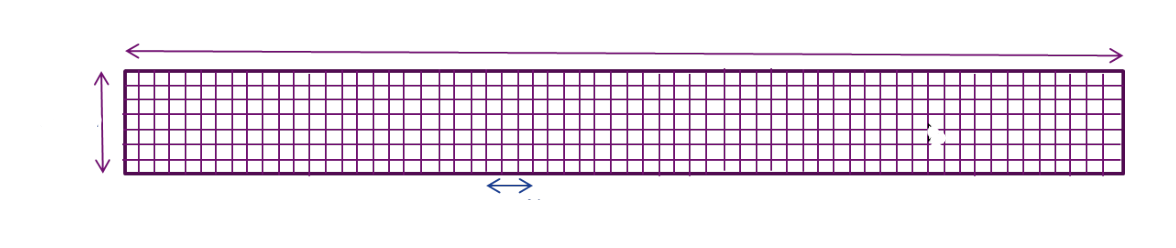
\includegraphics[scale=0.4]{images/chapter_3/schematic_GE.png}
\caption{Schematic of the solid material as an FDTD grid}
\end{center}
\end{figure}
\begin{figure}
\begin{center}
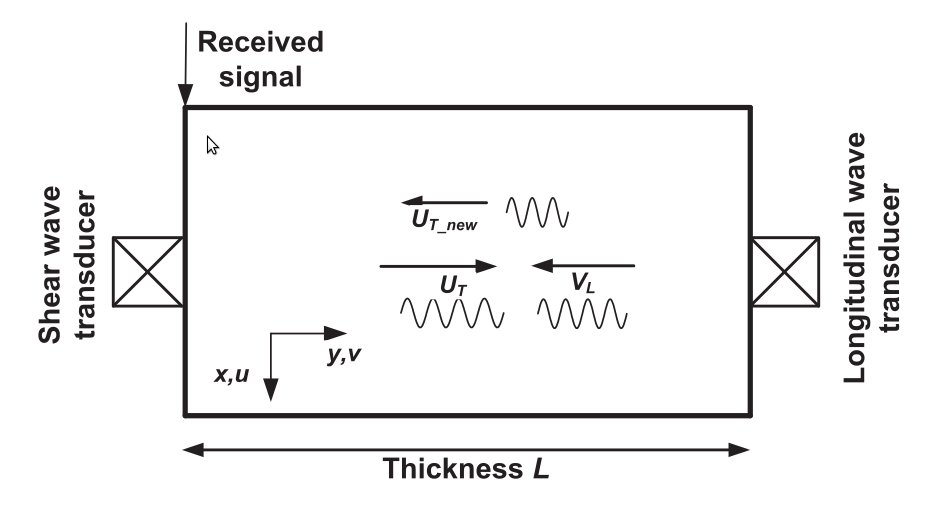
\includegraphics[scale=0.4]{images/chapter_3/schematic_liu.jpg}
\caption{Schematic of the setup the FDTD simulation is mimicking}
\end{center}
\end{figure}
\subsection{Numerical Considerations}
\subsubsection{Stability Criteria}
A finite difference scheme is stable if the errors made at one time step of the calculation do not cause the errors to increase as the computations are continued. A neutrally stable scheme is one in which errors remain constant as the computations are carried forward. If the errors decay and eventually damp out, the numerical scheme is said to be stable. If, on the contrary, the errors grow with time the numerical scheme is said to be unstable. The stability of numerical schemes can be investigated by performing von Neumann stability analysis. For time-dependent problems, stability guarantees that the numerical method produces a bounded solution whenever the solution of the exact differential equation is bounded. Stability, in general, can be difficult to investigate, especially when the equation under consideration is non-linear. \\
In the FDTD for sound waves, the main stability criteria is the \textbf{Courant} condition. This constraint ensures that the errors in the numerical simulation get damped out to give a fairly accurate  estimate of the actual solution.
\begin{equation}
\Delta t \leq \frac{1}{C} \frac{1}{\sqrt{\frac{1}{(\Delta x)^2}+\frac{1}{(\Delta y)^2}}}
\end{equation}
\begin{equation}
\Delta x = \Delta y,
\Delta t \leq \frac{1}{C} \frac{1}{\sqrt{2}}
\end{equation}
\subsubsection{Boundary Conditions}
The simulation needs a few boundary conditions to be set up, such that there is a solution to the equation that is solved. In this case, we assume the propagation of the wave as equal to the propagation of a wave through any standard wave guide. Since, we are assuming a metal-to-air interface, we have modeled this as a completely reflecting wave guide with no absorption. For other interfaces or absorption in the wave-guide, we could look at a Perfectly Matched Layers (PML) at the boundaries for complete absorption.

The wave guide is modeled as a free waveguide on all ends and the movement is not restricted anywhere. For such a scenario, in the case of plane wave propagation in solids, it is the particle displacement at the boundary which is free, and nothing else. In case the ends are not free to move, the particle displacements at the boundary are trivial. For both these cases, we see reflections, but there is a phase inversion that happens in the latter case. This is not of great importance in this context, but helps validate simulations.

The conditions for the same implemented in the code is as follows.
\begin{equation}
u^n_{-1} = u^n_{-2}
\end{equation}
\begin{equation}
v^n_{-1} = v^n_{-2}
\end{equation}
Where $-1, -2$ denote the grid points from the boundaries, with $-1$ being the last grid point.
\subsubsection{Initial condition}
Another important component of the boundary layer is basically the initial conditions of the simulation itself. This determines the initial state of the system and the excitement that is given to the system and determines the outcome of the simulation. 

For this FDTD simulation, we need to excite the system with one transverse and one longitudinal wave on either end. As the system we have currently taken is collinear, the only criteria is the excitation, and nothing else. The initial wave forms must also be smooth\cite{smoothness} to prevent numerical dispersion and dissipation errors in the simulations \cite{errors} \cite{errors_2}

\textbf{Mesh and Sampling Sampling}
To further get a more accurate solution, we have to choose a suitable size of mesh for which the solution is acceptable and at the same time not too time consuming. The solution must be approximately right, without too much noise in the data. The solution is also sampled at a rate which is extremely high to prevent aliasing of the data. We sample at a rate that is proportional to the meshing, a criteria we get from the courant condition.

\section{Simulation}
\subsection{Sources}
There are two main sources in the simulations, one is a longitudinal wave with a specific frequency and another is a transverse wave coming in from the opposite direction. These are limited in time, and thus are pulses of waves. The pulses are raised cosine pulses with a pulse width of 10. 
\begin{figure}
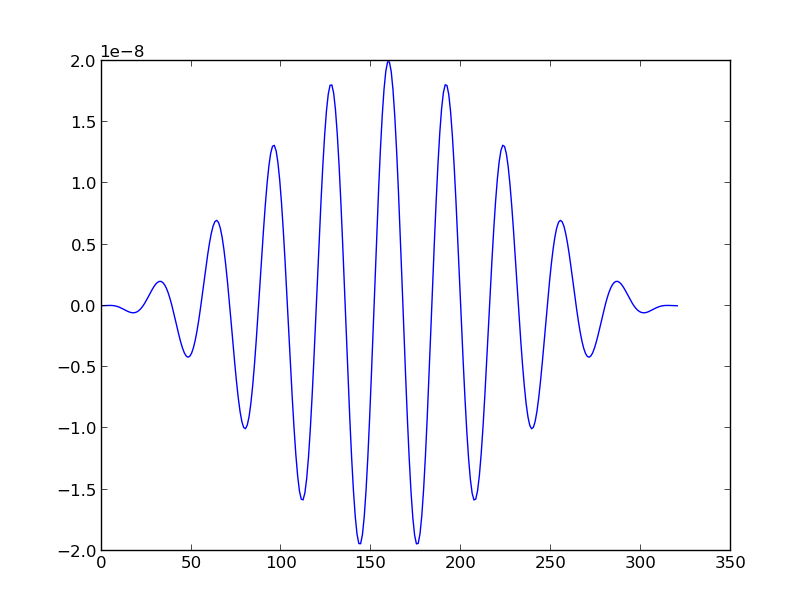
\includegraphics[scale=0.5]{images/chapter_3/wave_1.png}
\caption{Longitudinal Pulse Excited at Source}
\end{figure}
\begin{figure}
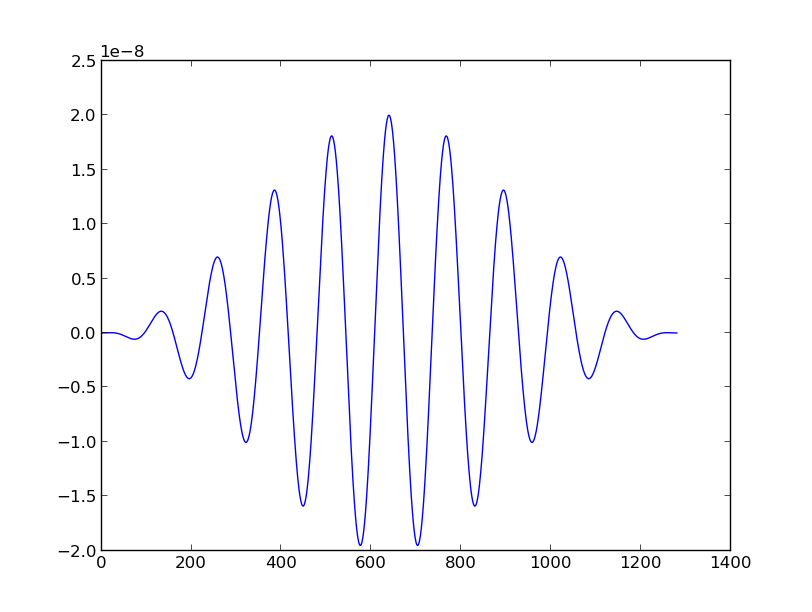
\includegraphics[scale=0.5]{images/chapter_3/wave_2.png}
\caption{Transverse Pulse Excited at Source}
\end{figure}
\subsection{Simulation Parameters}
\begin{table}[ht]
\caption{General Numerical Properties of Simulation}
\begin{tabular}{|c|c|}
\hline
\textbf{Property} & \textbf{Value} \\ \hline
$\Delta t$ & $3.125 \times 10^{-09}$s \\ \hline
$\Delta x$ & $3.94 \times 10^{-05}$m \\ \hline
Sampling Frequency & $3.2 \times 10^{8}$Hz \\ \hline
\end{tabular}
\end{table}
\begin{table}[ht]
\caption{Pulse Properties}
\begin{tabular}{|c|c|c|}
\hline
\textbf{Property} & \textbf{Longitudinal} & \textbf{Transverse} \\ \hline
Number of pulses & 10 & 10 \\ \hline
Pulse Frequency & 10MHz & 2.5MHz \\ \hline
Pulse Amplitude & $2 \times 10^{-8}$m & $2 \times 10^{-8}$m \\ \hline
Pulse Duration & $10^{-6}$s & $4 \times 10^{-6}$s \\ \hline
Pulse Velocity & $6299.5ms^{-1}$ & $3100ms^{-1}$\\ \hline 
\end{tabular}
\end{table}
\section{Simulation Results}
\subsection{Snapshots of Simulation}
\begin{figure}[ht]
\centering
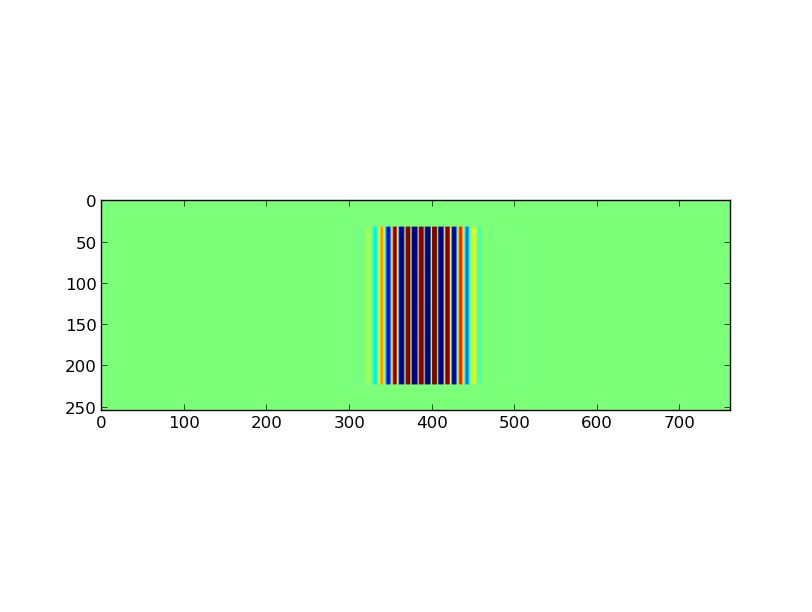
\includegraphics[scale=0.5]{images/chapter_3/simulation_picture_long.png}
\caption{Snapshot of the Longitudinal Wave}
\end{figure}

\begin{figure}[ht]
\centering
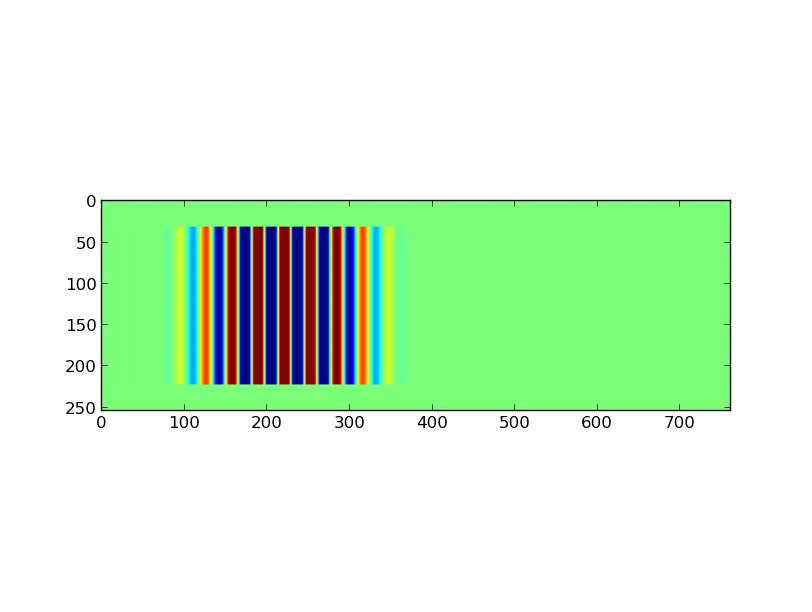
\includegraphics[scale=0.6]{images/chapter_3/simulation_picture_transverse.png}
\caption{Snapshot of the Transverse Wave}
\end{figure}

\begin{figure}[!ht]
\centering
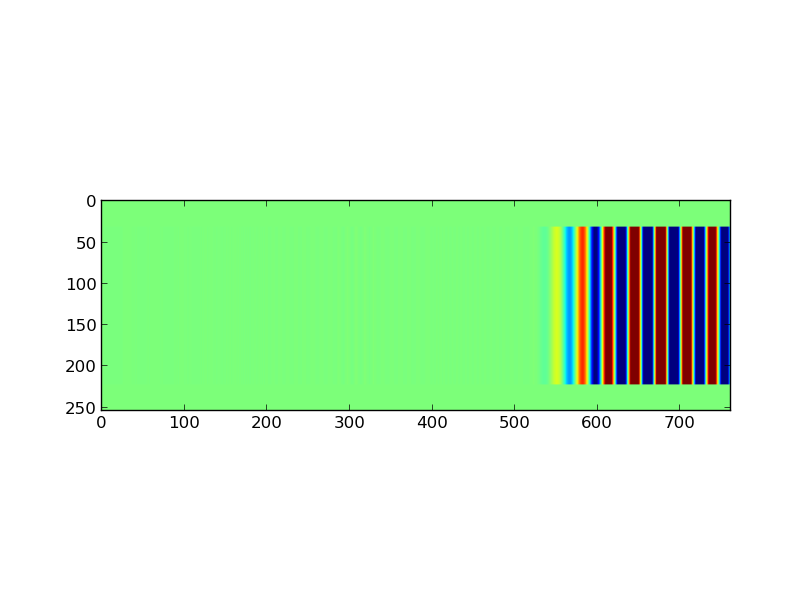
\includegraphics[scale=0.6]{images/chapter_3/wave_trans.png}
\caption{Snapshot of the Transverse Wave}

\end{figure}

\subsection{Validation of Simulation}
The solution from the simulation was obtained from an Amplitude Scan at both the sources. The wave forms and the fourier transforms of the waves after the A-scans were consistent with what is expected from an FDTD simulation. There was minimal dispersion or dissiparion error and thus the simulation parameters were satisfactory. To check if the FDTD simulation is accurate enough to be used for more complex cases with the same solver and engine, we compared the results of our FDTD simulation with the one by Liu Et. al \cite{Liu} which solved this case by the use of an ODE solver. 

From the comparisons of the two solutions, we compared the scale of amplitude as well as the frequency of the generated wave. Due to our input being markedly different from that of the reference paper, the deviations in wave shape are acceptable. All the other criteria match with that of the reference paper. The comparisons and Validation plots are given below.


\begin{figure}[ht]
\begin{center}
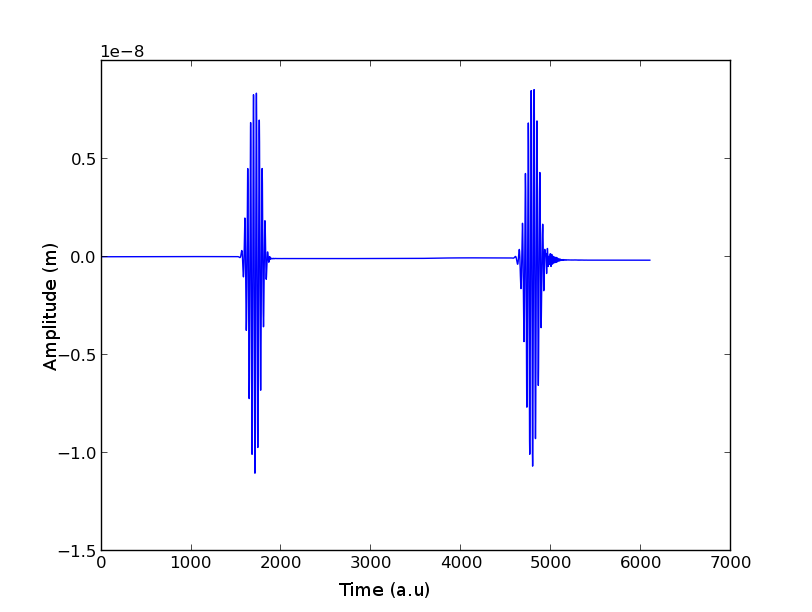
\includegraphics[scale=0.7]{images/chapter_3/final_longitudinal.png}
\caption{A-scan of the longitudinal wave}
\end{center}
\end{figure}

\begin{figure}[ht]
\begin{center}
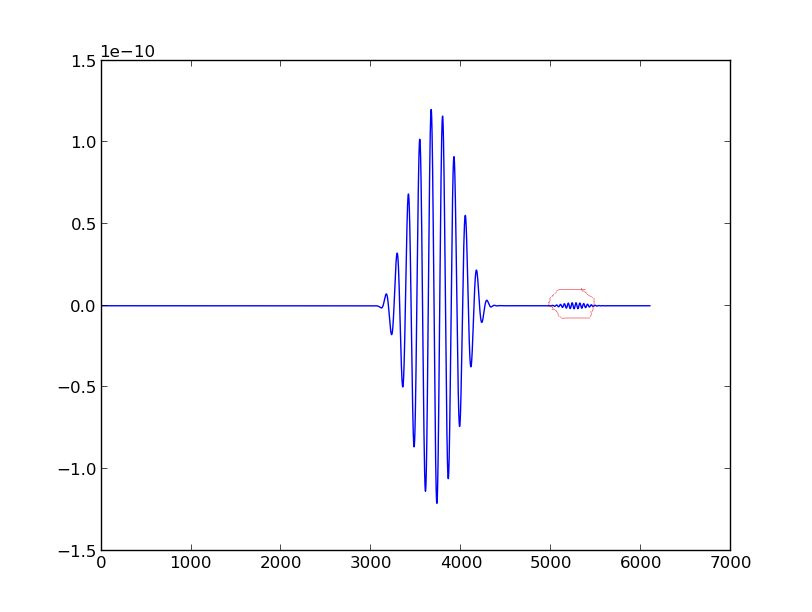
\includegraphics[scale=0.5]{images/chapter_3/final_transverse.png}
\caption{A-scan of the transverse wave}
\end{center}
\end{figure}

\begin{figure}[ht]
\begin{center}
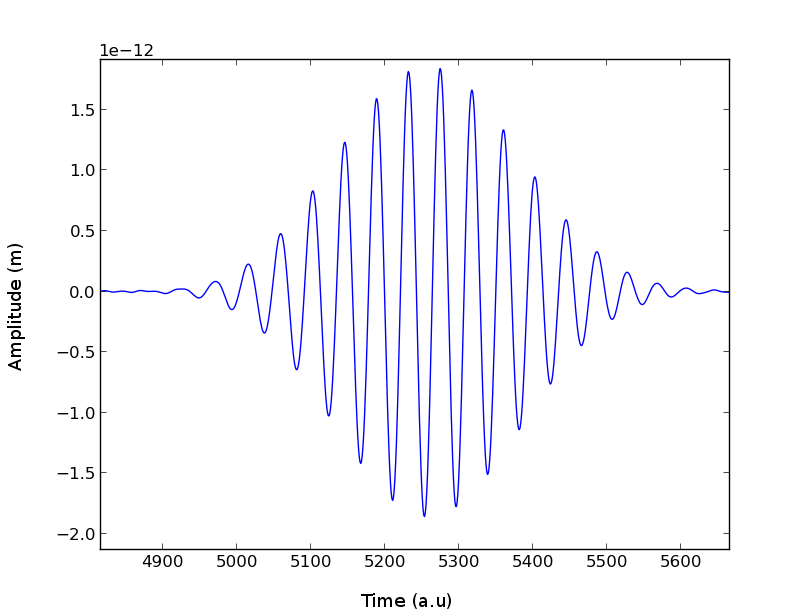
\includegraphics[scale=0.5]{images/chapter_3/final_transervse_zoom.png}
\caption{Zoomed A-scan of transverse wave}
\end{center}
\end{figure}


\begin{figure}
\begin{center}
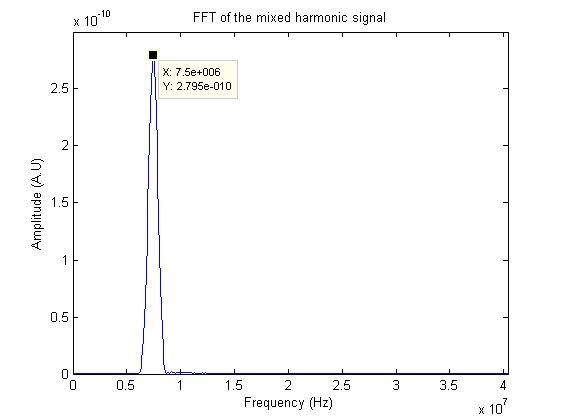
\includegraphics[scale=0.5]{images/chapter_3/finaLfft_zzom.jpg}
\caption{Fourier Transform of the New Wave Generated}
\end{center}
\end{figure}

\begin{figure}
\begin{center}
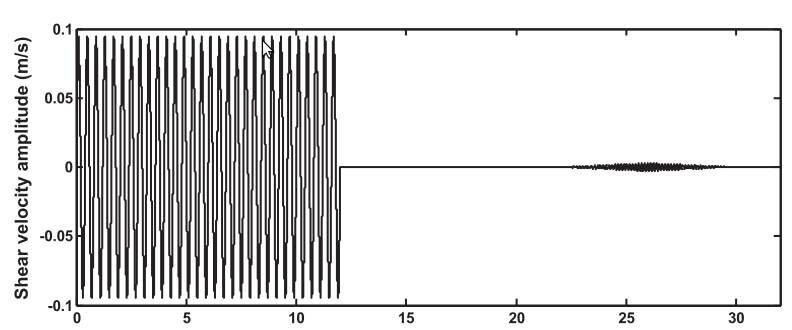
\includegraphics[scale=0.5]{images/chapter_3/validation.png}
\caption{Simulation Results From DE solver\cite{Liu}}
\end{center}
\end{figure}

\begin{figure}
\begin{center}
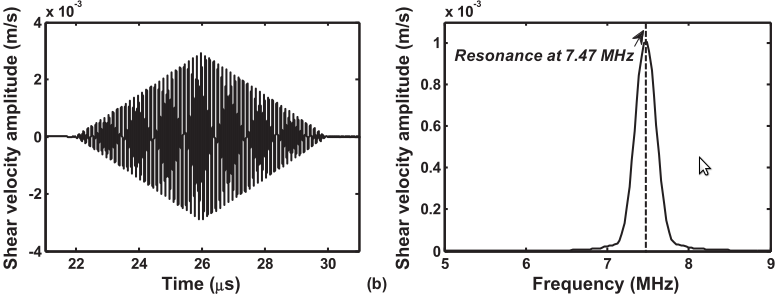
\includegraphics[scale=0.5]{images/chapter_3/validation_2.png}
\caption{Zoomed solution and Fourier Transform of the solution from DE solver \cite{Liu}}
\end{center}
\end{figure}